\documentclass[11pt,a4paper,twocolumn]{article}
\usepackage[utf8]{inputenc}
\usepackage[T1]{fontenc}
\usepackage{amsmath}
\usepackage{amsfonts}
\usepackage{amssymb}
\usepackage{graphicx}
\usepackage{hyperref}
\usepackage{cleveref}

\usepackage{natbib}

\hypersetup{
	colorlinks=true,
	linkcolor=blue,
	filecolor=magenta,      
	urlcolor=cyan,
}


\author{Karl Kristian Ladegård Lockert}
\title{TFY4235: Exam}
\begin{document}
\maketitle
\begin{abstract}
	
	Exam solutions for TFY4235: Computational physics spring 2020.
	
\end{abstract}
		
\section{Assignment 2}
The final report for Assignment 2: Biased Brownian motion are attached together with code for the project. The core functionality of the program is written in Python, with heavy utilisation of compiled packages, as well as functionality for compiling python code. Most plots and development have been done in Jupyter Notebooks, which can be found in the Notebooks folder. If you do not have a Notebook viewer available, the very same files can be found and viewed in my open \href{https://github.com/kklocker/NumFys}{GitHub repository}. These files are, however, much more experimental and less documented, as they are created for very specific tasks or testing. The repository also contains additional plots, but these should be looked upon with great caution; if they are not included in the report there is no guarantee that the represent actual results rather than tests for different functions. 

\section{Ising model and Mon-Jasnow algorithm}

The first three days of the home exam have been spent debugging erroneous results produced by the original Mon-Jasnow algorithm. Discussing with TA's have both been helpful, but also a bit frustrating due to miscommunications on both parts. There has been good clarification in what to expect from the results, but the interpretation of the ensemble average showed to be trickier. 
Including the mixed messages of the factor 2, which at the start was a relief giving better results for $\tau$, but was later changed. After discussions with several other students, I believe the fundamental difference in my interpretation (which would not have a factor two) is in the interpretation of the Hamiltonians $H_{++}$ and $H_{+-}$, a problem many other students also have had. 
In the end, neither the results with $J$ scaled by a factor 2, nor the ``correct'' interpretation gave good results. 
\begin{figure}
	\centering
	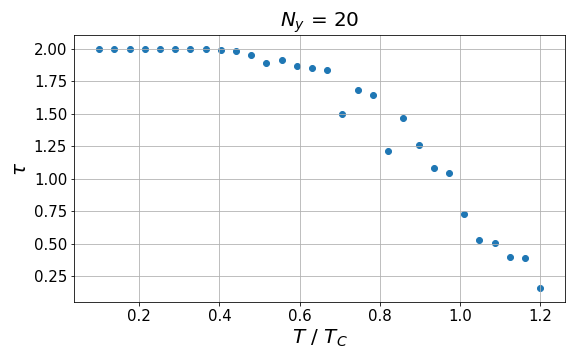
\includegraphics[width=\linewidth]{img/Ny20_Sweeps20000_Nruns1_Skips3_Nsteps30}
	\caption{The original Mon-Jasnow algorithm. For $N_y = 20$. The simulation was done with 20000 sweeps of $N^2$ spin-flip tries.}
	\label{fig:ny20sweeps20000nruns1skips3nsteps30}
\end{figure}
I finally started implementing the torus and Klein-bottle boundary conditions when the results were decent, although I am not pleased with the outcome, presented in \cref{fig:ny20sweeps20000nruns1skips3nsteps30}.
The shape is reminiscent of that in . By interpreting the Hamiltonian in the other way, we get a curve that is going to 0 at $T = T_C$, but has the wrong shape. This is viewed in \cref{fig:ny100sweeps2000nruns1skips3}. Extrapolating the ``correct' shape from the low-$T$ data points, we end up with a ``critical temperature'' at $T \simeq 0.65T_C$. 
\begin{figure}
	\centering
	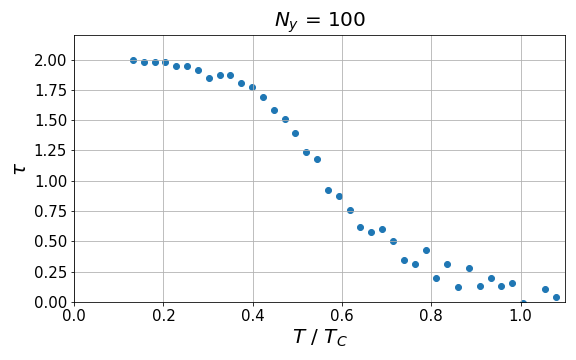
\includegraphics[width=\linewidth]{img/Ny100_Sweeps2000_Nruns1_Skips3}
	\caption{The original Jon-Masnow algorithm for $N_y$ =100 with 2000 sweeps of $N^2$ spin flip tries. Here $J$ is scaled by a factor two, by interpreting the Hamiltonians differently.}
	\label{fig:ny100sweeps2000nruns1skips3}
\end{figure}

\bibliographystyle{unsrt}
\bibliography{./bib.bib}
\end{document}

